% How we do it: Why we do it, What particular method we use and what logic architecture we use
\section{The methodological approach}
\label{MethodApproach}
%---What methodology we used---

We analyze the possibility of automatically transform a BPEL written process in a Java executable routine, with minimum ad-hoc developer’s intervention. Our final objective is to show the feasibility of a semi-automated transformation from a small business process orchestrated with BPEL to the Java language.
This section describes the methodological approach we undertaken to realize our objective. The steps are summarized as following:

\begin{itemize}
 \item We identify the subset of BPEL instructions suitable for a proof of concept of the transformation.
 \item Select a BPEL meta-model that covers the chosen subset of instructions.
 \item Individuate a BPEL workflow pattern to work on
 \item Choose a model driven methodology that allows us to manipulate  the BPEL input model (M2M, M2T) and that is compatible with a ready to run code output.
\end{itemize} 

Once these steps have been accomplished, we focus on providing more details on how we carry out the transformation. The main points are:
\textbf{DA SCRIVERE NELLA SEZIONE DETAILED ARCHITECTURE ? }
\begin{itemize}
 \item Provide a correspondence from BPEL constructs to Java concepts
 \item Design the structure of the output application.
 \item Define the essential skeleton of Java classes necessary to create a runnable BPEL process
 \item In the templates, describe how to use and where the dynamic information taken from the BPEL input model has to be placed.
 \item Plan where and how, in the architecture, the developer intervention has to take place.
 \item \textbf{Issues encountered and proposed solutions  ? }
\end{itemize} 
 
 To mention later: \\
 StubPartnerLinks, code to be input by the user, static code, the problem with the WSDL file

\subsection{The BPEL subset of instructions}
\label{Sec:BPELsubset}
The BPEL standard (see Section \ref{BPEL} for more details) has a wide variety of elements and instructions aimed at managing the possible workflow patterns obtainable during a services orchestration. Moreover, BPEL does not restrict the number of services that can participate to the orchestration neither the type and the quantity of interactions among them.
For these reason, we focus our attention on a subset of the whole BPEL language, both to restrain the complexity and to fit the time frame of the project.
\subsubsection{The activities subset}
We decided to restrict the BPEL activities to a subset containing the following constructs divided in four groups:
\begin{center}
\begin{supertabular}{p{0.4\textwidth}p{0.4\textwidth}}

1. Basic activities: 			& 2. Structured activities:		\\
\begin{itemize}
	\item \verb|<invoke>|
	\item \verb|<receive>|
	\item \verb|<reply>|
	\item \verb|<assign>|
	\end{itemize} 			&

					    \begin{itemize}
					      \item \verb|<sequence>|
					     \end{itemize}			\\
					     
3. Elementary operations: 		& 4. Static descriptive elements:	\\					
\begin{itemize}
	\item \verb|<copy>|
	\item \verb|<from>|
	\item \verb|<to>|
  \end{itemize} &

					    \begin{itemize}
					      \item \verb|<process>|
					      \item \verb|<partnerLink>|
					      \item \verb|<variable>|
					      \item \verb|<expression>|
					    \end{itemize}\\
\end{supertabular}
\end{center}

These elements allow the creation of simple BPEL processes, where the activities such as: invoking a service or waiting for a reply, happen as a sequence, one after the other. Although this limits the expressive potentiality of BPEL, it fits our need of focusing on proving the feasibility of an automated transformation from BPEL to Java without having to deal with the complexity of the whole language.
In Figure \ref{fig:SubSetBPEL} the BPEL subset of elements used for this project is depicted.

\begin{figure}
  \begin{center}
    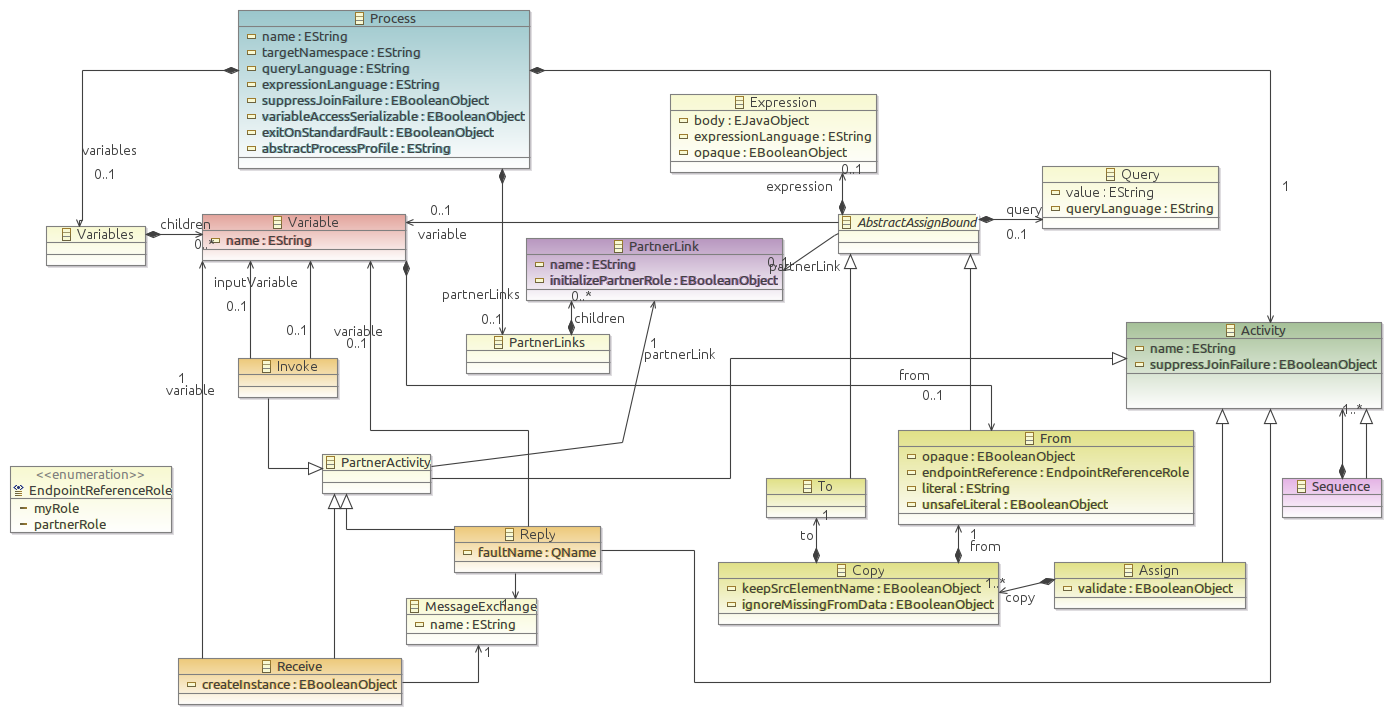
\includegraphics[scale=0.67,angle=90]{pictures/SubSetBpel2.png}
    \caption{The BPEL subset in its ecore model representation}
    \label{fig:SubSetBPEL}
  \end{center}
\end{figure} 

\subsubsection{The meta-model for the BPEL subset}
\label{Sec:DesignBpelSubset}
To permit the parameterization of the BPEL process input model, we need a meta-model describing our subset. The Eclipse Modeling Framework (see Section \ref{EMF}) provides a meta-model written in ecore for the whole BPEL language; we use only the subset elements of this ecore meta-model.
\subsubsection{The BPEL workflow pattern to focus on}
\label{sec:DesignBPELPattern}
The BPEL language with its wide range of activities and operation, gives the possibility to orchestrate many kind of workflow patterns among the participant services. We concentrate our attention on a process having the following participants:
\begin{itemize}
 \item one partner link representing a client
 \item one partner link describing a web-service
\end{itemize}
and on a simple workflow pattern that concerns the activities shown in Figure: \ref{fig:BPELWorkflowPattern}\footnote{This Figure has been realized using the BPEL designer facilities of Eclipse. Yet not a standard, as the Oasis consortium has not released a graphical standard, many vendors provide very similar graphical notations}. The pattern shown in the Figure includes the following steps:
\begin{enumerate}
 \item the process waits for a client to connect and provide an input
\item reception of the input and its assignation to a variable to forward to the web-service.
\item web-service invocation
\item reception of the web-service's reply and assignation to a variable to be forwarded back to the client
\item final response sent back to the client
\end{enumerate}


\begin{figure}
  \begin{center}
    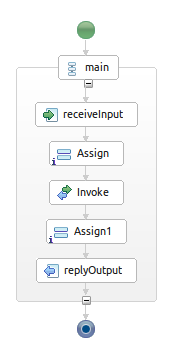
\includegraphics[scale=0.8]{pictures/BPELSimpleProcess.png}
    \caption{The BPEL workflow pattern we focus on}
    \label{fig:BPELWorkflowPattern}
  \end{center}
\end{figure} 
% %\lipsum[2]
% \hvFloat[
%  floatPos=!htb,
%  capWidth=h,
%  capPos=r,
%  capAngle=90,
%  objectAngle=90,
%  capVPos=c,
%  objectPos=c]{figure}{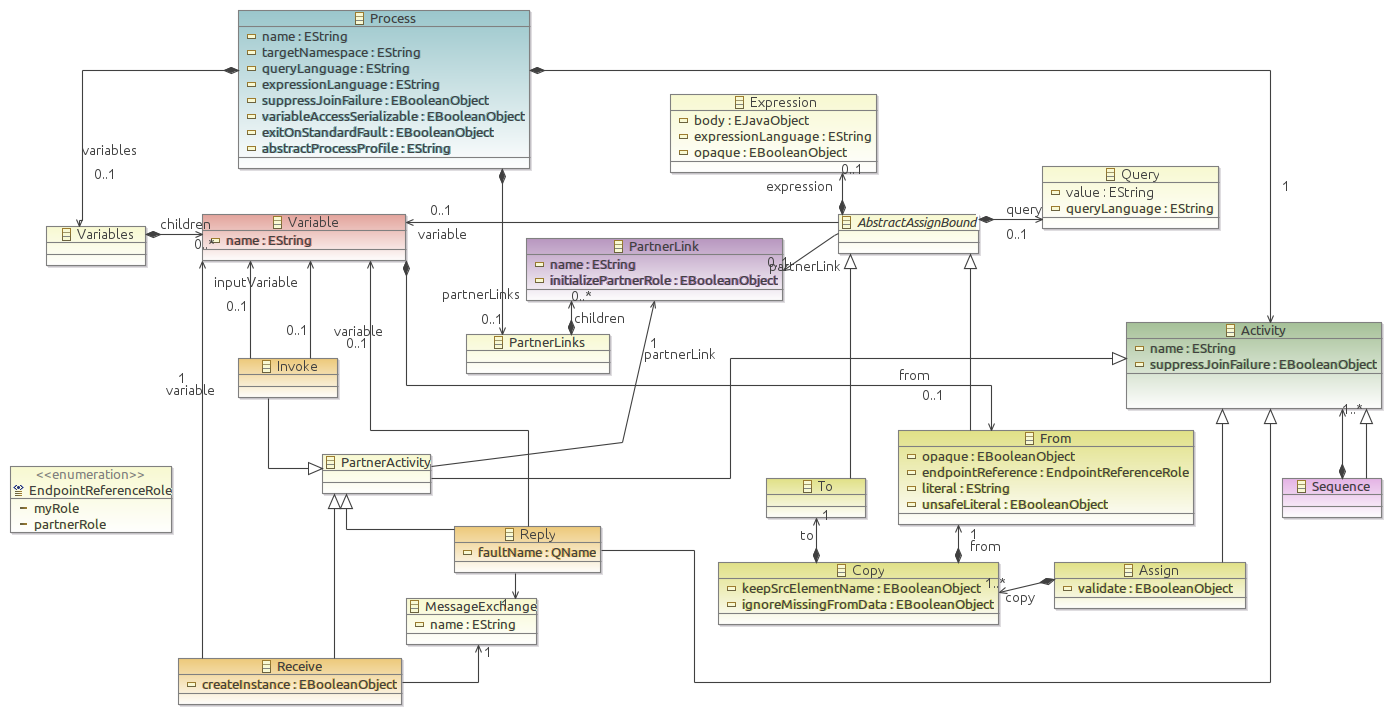
\includegraphics[scale=0.7]{pictures/SubSetBpel2.png}}%
% {Caption vertically centered right beside the float with a caption
% width of figure width and 
% \texttt{floatcapsep=5pt} (the default)}{fig:label}


\begin{figure}
  \begin{center}
    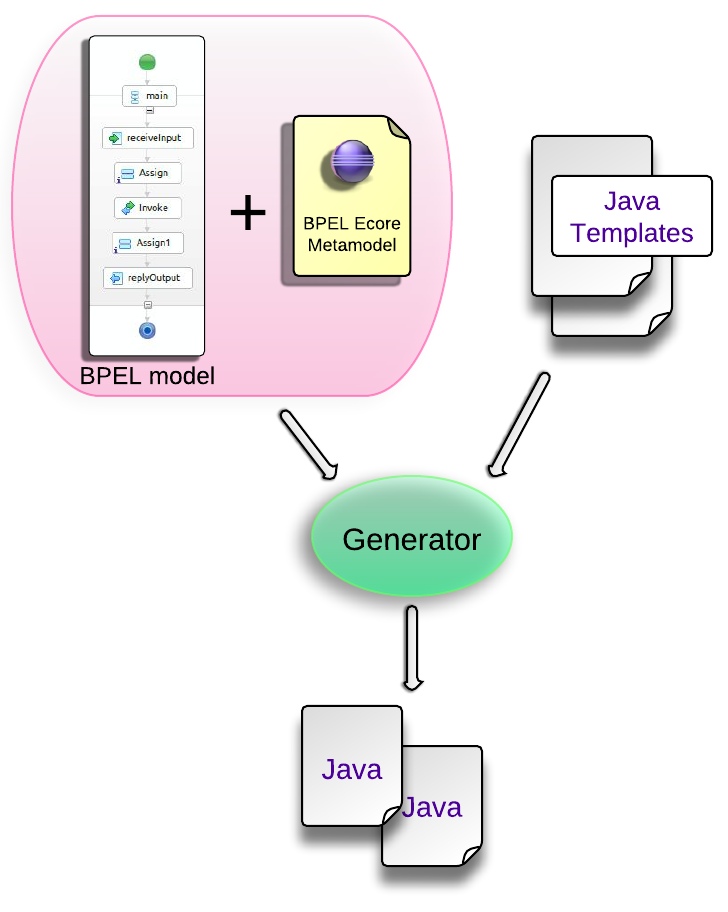
\includegraphics[scale=0.9]{pictures/TransformationApproach.png}
    \caption{The methodological transformation approach}
    \label{fig:TransformationApproach}
  \end{center}
\end{figure}

%----------------------------------------------------


% \begin{multicols}{2}
% \begin{enumerate}
%     \item Basic activities:
%     \begin{itemize}
% 	\item \verb|<invoke>|
% 	\item \verb|<receive>|
% 	\item \verb|<reply>|
% 	\item \verb|<assign>|
% 	\end{itemize}
%     \item Structured activities: 
%     \begin{itemize}
% 	\item \verb|<sequence>|
%     \end{itemize}
%     \item  Elementary operations:
%     \begin{itemize}
% 	\item \verb|<copy>|
% 	\item \verb|<from>|
% 	\item \verb|<to>|
%     \end{itemize}
%     \item Static descriptive elements:
%     \begin{itemize}
% 	\item \verb|<process>|
% 	\item \verb|<partnerLink>|
% 	\item \verb|<variable>|
% 	\item \verb|<expression>|
%     \end{itemize}
% \end{enumerate}
% \end{multicols}